%!TEX root = twig.tex

\subsection{Operators}
\label{sec:semantics:ops}

Expressions can be combined using Twig's operators. In the
following semantics, let $t$ range over terms, $m$ range over
blocks, and $s$ range over expressions, i.e., either a primitive
rule, or else another expression built with operators.

The \emph{sequence} operator, written as an infix semi-colon
(\texttt{;}), chains the application of two rules together by
sending the output of the first to the input of the second. The
combined expression fails if either sub-expression fails. With
this operator, simple rules can be composed into multi-step
transformations. Upon success, the result blocks are combined
sequentially using the block sequence operation (see
Section~\ref{sec:code-gen:seq}). The formal semantics are:

\begin{equation}
\label{S1}
\infer
  {t \arr{s_1;s_2} (t'',m_1+m_2)}
  {t \arr{s_1} (t',m_1) \quad t' \arr{s_2} (t'',m_2)}  
\end{equation}

\begin{equation}
\label{S2}
\infer
  {t \arr{s_1;s_2} \bot}
  {t \arr{s_1} \bot}  
\end{equation}

\begin{equation}
\label{S3}
\infer
  {t \arr{s_1;s_2} \bot}
  {t \arr{s_1} (t',m) \quad t' \arr{s_2} \bot}  
\end{equation}

The sequence operator is associative, that is for any expressions
$f,g,h$, $(f;g);h$ is equivalent to $f;(g;h)$. This allows us to
write expressions like $f;g;h$ without ambiguity. We prove this
fact in Section~\ref{sec:seq-assoc}.

\emph{Left-biased choice}, written as a vertical bar (\texttt{|}),
will attempt to apply the first rule expression to the input, and
if it succeeds then its output is the result. If it fails, it
attempts to apply the second rule instead. This operator allows
different code to be generated depending on the input type.
Formally:

\begin{equation}
\label{C1}
\infer
  {t \arr{s_1|s_2} (t',m_1)}
  {t \arr{s_1} (t',m_1)}
\end{equation}

\begin{equation}
\label{C2}
\infer
  {t \arr{s_1|s_2} (t',m_2)}
  {t \arr{s_1} \bot \quad t \arr{s_2} (t',m_2)}
\end{equation}

\begin{equation}
\label{C3}
\infer
  {t \arr{s_1|s_2} \bot}
  {t \arr{s_1} \bot \quad t \arr{s_2} \bot}
\end{equation}

Like the sequence operators, left-biased choice is associative.
For any expression $f,g,h$, $(f|g)|h$ is equivalent to $f|(g|h)$,
allowing us to write $f|g|h$ without ambiguity. We prove this fact
in Section~\ref{sec:choice-assoc}.

Twig includes a variety of other basic operators. The
\emph{identity} (\texttt{T}) expression will always succeed,
returning its input and an identity block. Conversely,
\emph{failure} (\texttt{F}) will always return \texttt{$\bot$}.

\begin{equation}
\label{SUCC}
\infer
  {t \arr{\mathtt{T}} (t,I)}
  {}  
\end{equation}

\begin{equation}
\label{FAIL}
\infer
  {t \arr{\mathtt{F}} \bot}
  {}  
\end{equation}

The unary operator \emph{test} (\texttt{?}) succeeds only if its
argument succeeds, returning the original term and discarding the
result term and block. This operator is useful for examining a
term's structure without actually making use of its sub-terms.

\begin{equation}
\infer
  {t \arr{?s} (t,I)}
  {t \arr{s} (t',m)}
\end{equation}

\begin{equation}
\infer
  {t \arr{?s} \bot}
  {t \arr{s} \bot}  
\end{equation}

Negation (\texttt{$\lnot$}) also takes a single expression
argument. It succeeds only if its argument fails on the input,
returning the original term.

\begin{equation}
\infer
  {t \arr{\lnot s} \bot}
  {t \arr{s} (t',m)}  
\end{equation}

\begin{equation}
\infer
  {t \arr{\lnot s} (t,I)}
  {t \arr{s} \bot}  
\end{equation}

Twig also provides some operators especially for tuples.

The \emph{congruence} operator applies a tuple of expressions to
the elements of a tuple term, pairwise, and returns a tuple of
results. It fails in case any of the individual rule applications
fail. Upon success, the result block is the parallel composition
(see Section~\ref{sec:code-gen:par}) of the individual result
blocks. The formal semantics are as follows:

\begin{equation}
\label{T1}
\infer
  {\mathtt{tuple}(t_1,\ldots,t_n) \arr{(s_1,\ldots,s_n)} (\mathtt{tuple}(t_1',\ldots,t_n'),m_1 \times \ldots \times m_n)}
  {t_1 \arr{s_1} (t_1',m_1) \quad \cdots \quad t_n \arr{s_n} (t_n',m_n)}
\end{equation}

\begin{equation}
\label{T2}
\infer
  {\mathtt{tuple}(\ldots,t_i,\ldots)\arr{(\ldots,s_i,\ldots)}\bot}
  {t_i \arr{s_i} \bot}
\end{equation}

\begin{equation}
\label{T3}
\infer
  {\mathtt{tuple}(t_1,\ldots,t_m) \arr{(s_1,\ldots,s_n)} \bot 
   \quad\mbox{if}\; m \neq n}
  {}
\end{equation}

\begin{equation}
\label{T4}
\infer
  {t \arr{(s_1,\ldots,s_n)} \bot
  \quad\mbox{if}\; t \neq \mathtt{tuple}(\ldots)}
  {}  
\end{equation}


The family of unary \emph{branch} operators apply a single
expression to one, all, or some of a tuple's elements, depending
on the variant.

The branch operator \texttt{\#one} attempts to apply its parameter
$s$ to a single element: the first element, from left to right,
for which $s$ does not fail. The other elements of the tuple are
unchanged. The expression fails if $s$ fails for each element. The
formal semantics for \texttt{\#one} are as follows:

\begin{equation}
\infer
  {\mathtt{tuple}(\ldots,t_i,\ldots) \arr{\mathtt{\#one}(s)} (\mathtt{tuple}(\ldots,t_i',\ldots),(I \times \ldots \times m_i \times \ldots \times I))}
  {t_i \arr{s} (t_i',m_i)}
\end{equation}

\begin{equation}
\infer
  {\mathtt{tuple}(t_1,\ldots,t_n) \arr{\mathtt{\#one}(s)} \bot}
  {t_1 \arr{s} \bot \quad \cdots \quad t_n \arr{s} \bot}  
\end{equation}

\begin{equation}
\infer
  {t \arr{\mathtt{\#one}(s)} \bot
  \quad\mbox{if}\; t \neq \mathtt{tuple}(\ldots)}
  {}  
\end{equation}


The branch operator \texttt{\#all} applies its parameter $s$ to
each element of a tuple. The expression fails if $s$ fails for any
element. The formal semantics for \texttt{\#all} are:

\begin{equation}
\infer{
  \mathtt{tuple}(\ldots,t_i,\ldots)
  \arr{\mathtt{\#all}(s)}
  (\mathtt{tuple}(\ldots,t_i',\ldots),
  (m_1 \times \ldots \times m_n))
}{
  t_1 \arr{s} (t_1',m_1) \quad \cdots \quad t_n \arr{s} (t_n',m_n)
}
\end{equation}

\begin{equation}
\infer
  {\mathtt{tuple}(\ldots,t_i,\ldots) \arr{\mathtt{\#all}(s)} \bot}
  {t_i \arr{s} \bot}  
\end{equation}

\begin{equation}
\infer
  {t \arr{\mathtt{\#all}(s)} \bot
  \quad\mbox{if}\; t \neq \mathtt{tuple}(\ldots)}
  {}  
\end{equation}


The branch operator \texttt{\#some} applies its parameter $s$ to
at least one element of a tuple. The expression fails if $s$ fails
for each elements. The formal semantics for \texttt{\#some} are:

\begin{equation}
\infer{
  \mathtt{tuple}(t_1,\ldots,t_n)
  \arr{\mathtt{\#some}(s)}
  (\mathtt{tuple}(P(t_1),\ldots,P(t_n)),
   Q(t_1) \times \ldots \times Q(t_n))
}{
\begin{array}{l}
P(t) = \left\{
  \begin{array}{l l}
    t' & \quad \text{if}\; t \arr{s} (t',m) \\
    t  & \quad \text{if}\; t \arr{s} \bot \\
  \end{array}\right.\\
Q(t) = \left\{ 
  \begin{array}{l l}
    m & \quad \text{if}\; t \arr{s} (t',m) \\
    I & \quad \text{if}\; t \arr{s} \bot \\
  \end{array}\right.\\
\exists{i} : i \in \{1..n\} \;\wedge\; t_i \arr{s} (t'_i,m)\\
\end{array}
}
\end{equation}

\begin{equation}
\infer
  {\mathtt{tuple}(t_1,\ldots,t_n) \arr{\mathtt{\#some}(s)} \bot}
  {t_1 \arr{s} \bot \quad \cdots \quad t_n \arr{s} \bot}
\end{equation}

\begin{equation}
\infer
  {t \arr{\mathtt{\#some}(s)} \bot
  \quad\mbox{if}\; t \neq \mathtt{tuple}(\ldots)}
  {}  
\end{equation}


A \emph{projection} extracts a single indexed element from a
tuple, discarding the other tuple elements. The formal semantics
are:

\begin{equation}
\infer
  {\mathtt{tuple}(\ldots,t_i,\ldots) \arr{\#i} (t_i,\Pi(i))}
  {}  
\end{equation}

\begin{equation}
\infer
  {\mathtt{tuple}(t_1,\ldots,t_n) \arr{\#i} \bot
  \quad\mbox{if}\; i > n}
  {}  
\end{equation}

\begin{equation}
\infer
  {t \arr{\#i} \bot
  \quad\mbox{if}\; t \neq \mathtt{tuple}(\ldots)}
  {}  
\end{equation}

The \emph{path} unary operator applies a rule to a single
indexed tuple element, leaving the other elements unchanged.

\begin{equation}
\infer
  {\mathtt{tuple}(\ldots,t_i,\ldots) \arr{\#i(s)} (\mathtt{tuple}(\ldots,t_i',\ldots), I \times \ldots \times m_i \times \ldots \times I)}
  {t_i \arr{s} (t_i',m_i)}
\end{equation}

\begin{equation}
\infer
  {\mathtt{tuple}(\ldots,t_i,\ldots) \arr{\#i(s)} \bot}
  {t_i \arr{s} \bot}
\end{equation}

\begin{equation}
\infer
  {\mathtt{tuple}(t_1,\ldots,t_n) \arr{\#i(s)} \bot
  \quad\mbox{if}\; i > n}
  {}  
\end{equation}

\begin{equation}
\infer
  {t \arr{\#i(s)} \bot
  \quad\mbox{if}\; t \neq \mathtt{tuple}(\ldots)}
  {}  
\end{equation}

The \emph{permutation} operator allows arbitrary permutation of a
tuple's elements, including duplicating or dropping elements. The
operator is parameterized by the width of the input tuple and a
list of indices into the tuple. The output will rearrange the
elements of the tuple in the order of the indices. The expression
will fail if the input does not have the given width, or if the
input is not a tuple.

\begin{equation}
\begin{array}{c}
\infer
  {\mathtt{tuple}(t_1,\ldots,t_n) \arr{\mathtt{\#permute}_n(x_1,\ldots,x_m)} (\mathtt{tuple}(t_{x_1},\ldots,t_{x_m}),\Pi_w(y_{x_1},\ldots,y_{x_m}))}{}\\
\mbox{where}\\
\begin{array}{rll}
    & & \{x_1..x_m\} \in \mathbb{N}\\
w   &=& \sum_{j=1}^n \mbox{width}(t_i)\\
b_i &=& \left\{
  \begin{array}{cl}
    0 & \mbox{if } i = 1\\
    \sum_{j=1}^{i-1} \mbox{width}(t_i) & \mbox{if } i > 1
  \end{array}
\right.\\
y_i &=& b_i+1,\ldots,b_i + \mbox{width}(t_i)
\end{array}
\end{array}
\end{equation}

\begin{equation}
\infer
  {\mathtt{tuple}(t_1,\ldots,t_m) \arr{\#\mathtt{permute}_n(\ldots)} \bot
  \quad\mbox{if}\; m \neq n}
  {}  
\end{equation}

\begin{equation}
\infer
  {t \arr{\#\mathtt{permute}_n(\ldots)} \bot
  \quad\mbox{if}\; t \neq \mathtt{tuple}(\ldots)}
  {}  
\end{equation}

The \texttt{\#permute} operator has relatively complex rules for constructing
the result block. This is because blocks must account for each element of a
tuple with a separate input and output. The \texttt{\#permute} operator, by
contrast, rearranges the top-level tuple but must preserve the ordering of
elements within sub-tuples. Figure~\ref{fig:permute} shows the application of
$\mathtt{\#permute}_4(4,3,2,1)$ to the tuple term $((t1,t2,t3),t4,(t5,t6),t7)$
-- the top-level tuple elements are permuted, while in the interior tuples,
ordering is preserved.

\begin{figure}[ht]
\centering
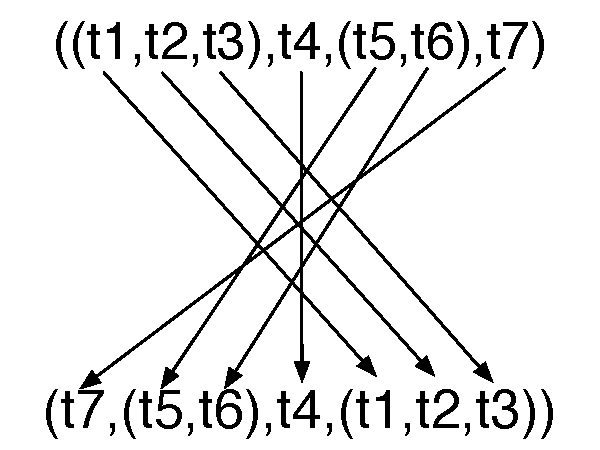
\includegraphics[width=2in]{images/permute}
\caption{Permutation of tuples.}
\label{fig:permute}
\end{figure}

The \texttt{\#fan} operator takes a integer parameter $n$, and
replicates the input term $n$ times in an $n$-element tuple. It is
similar to \texttt{\#permute} but does not require that its input
be a tuple.

\begin{equation}
\begin{array}{c}
\infer
  {t \arr{\mathtt{\#fan}(n)} (\mathtt{tuple}(t,\overset{n}{\ldots},t),\Pi_w(y,\overset{n}{\ldots},y))}
  {}\\
\mbox{where}\\
w = \mbox{width}(t)\\
y = 1,\ldots,w
\end{array}
\end{equation}

The fixed-point operator, \texttt{\#fix}, allows Twig to express
rules for handling recursively defined data types like lists and
trees. An application of $x$ within the expression
$\mathtt{\#fix}_x(s)$, that is, $x$ appearing within $s$, is
essentially a recursive call to the expression
$\mathtt{\#fix}_x(s)$.

\begin{equation}
\infer
  {t \arr{\mathtt{\#fix}_x(s)} (t',m)}
  {t \arr{s[x \mapsto \mathtt{\#fix}_x(s)]} (t',m)}
\end{equation}

\begin{equation}
\infer
  {t \arr{\mathtt{\#fix}_x(s)} \bot}
  {t \arr{s[x \mapsto \mathtt{\#fix}_x(s)]} \bot}
\end{equation}
